\documentclass{article}

\usepackage[final]{corl_2023}
\usepackage{graphicx}
\usepackage{booktabs}
\usepackage{amsmath,amssymb}
\usepackage{xcolor}
\usepackage{multirow}
\usepackage{subcaption}

\graphicspath{{../figs/}}

% ---- drafting macros: remove before submission --------------------------------------------------
\newcommand{\todo}[1]{\textcolor{red}{[TODO: #1]}}
\newcommand{\upd}[1]{\textcolor{blue}{#1}}   % number that changes once the extra seeds finish
% -------------------------------------------------------------------------------------------------

\newcommand{\fas}{\textsc{FAS}}
\newcommand{\C}{\mathcal{C}}

\title{When Does Failure-Aware Sampling Help?\\Robust Diffusion Policy Fine-Tuning under Dynamics Disturbances}

\author{
  Jingshu Peng \And Binghong Chen \And Yi Ni \And Arshbir Banipal \And Zhenghao Jin \\
  Carnegie Mellon University \\
  \texttt{\{jingshup, \todo{andrew IDs}\}@andrew.cmu.edu}
}

\begin{document}
\maketitle

%===============================================================================
\begin{abstract}
Diffusion policies fine-tuned with reinforcement learning in a single nominal environment are brittle under changes in dynamics.
Domain randomization fixes part of this, but it spends most of its samples on conditions the policy already solves.
We study \emph{Failure-Aware Sampling} (\fas{}): during DPPO fine-tuning, training conditions are sampled in proportion to the policy's current failure rate on them.
On walker2d, \fas{} improves success over uniform domain randomization by 3.9 points on the training grid, 7.8 points on the hardest quarter of conditions and 4.0 points on held-out conditions; a learning-progress-gated variant raises these gains to 6.0, 14.0 and 6.2 points.
On halfcheetah the gain is smaller (2.9 points, $t=2.0$, 8 seeds); on hopper \fas{} gives no gain, and sparse rewards make it worse.
Our evidence points to \emph{learnability}: hopper's grid contains a disturbance no method learns, and on a grid without it \fas{} beats uniform sampling, as we predicted before training.
Critic error does not appear to be the bottleneck: \fas{} does not increase it in any setting we measured. A value-error-based curriculum (PLR) performs worse than uniform sampling.
\todo{one sentence on the LEGO results.}
\end{abstract}

\keywords{Diffusion policy, RL fine-tuning, Domain randomization, Curriculum}

%===============================================================================
\section{Introduction}
\label{sec:intro}

Diffusion policies trained by imitation~\citep{chi2023diffusion} can be improved further with on-policy RL. DPPO~\citep{ren2025dppo} treats the denoising chain as part of the MDP and fine-tunes it with PPO~\citep{schulman2017ppo}.
In practice this fine-tuning runs in a single nominal simulator. A deployed robot, however, faces payloads, surfaces and pushes that the nominal simulator does not contain.
In our experiments, a DPPO policy fine-tuned on nominal walker2d succeeds in only 33\% of episodes under held-out mass, friction and push disturbances.

The standard remedy is domain randomization (DR)~\citep{tobin2017dr,peng2018sim2real}: sample the dynamics uniformly from a set of conditions during training.
Uniform DR ignores what the policy already knows. On walker2d, uniform DR solves 24 of our 36 conditions to $>$80\% success, yet keeps spending two thirds of its samples on them.
On-policy RL makes this worse. PPO's batch is a fixed number of environment \emph{steps}, and episodes on hard conditions end early when the robot falls. Under uniform DR, the hardest third of the conditions therefore receives only 24--26\% of the training steps.

\textbf{Key idea.} \emph{Sample training conditions in proportion to how often the current policy fails on them.}
Failure is cheap to measure, needs no learned model, and points the on-policy gradient at the conditions where it is likely to be most informative.
The idea can also fail. A failed condition may be unlearnable, and concentrating on it then wastes samples. Concentration may also destabilize the critic, which must track a moving state distribution, especially when the reward is sparse.

We therefore ask three research questions:
\textbf{(RQ1)} Does \fas{} improve robustness and sample efficiency over uniform DR?
\textbf{(RQ2)} What governs the trade-off between exploring hard conditions and training stability: sampling strength, reward sparsity, or critic error?
\textbf{(RQ3)} Is the RL update necessary, or does simply imitating the successes that RL discovered (rejection-sampling fine-tuning, RFT) suffice?

\textbf{Contributions.}
(i) A drop-in failure-aware condition sampler for DPPO, evaluated against uniform DR and three adaptive curricula (SGS, learning progress, PLR) on three MuJoCo tasks and a LEGO assembly task \todo{LEGO name}.
(ii) Evidence, including a prediction fixed before training, that the benefit of \fas{} depends on whether the failed conditions are learnable rather than on critic stability.
(iii) A negative result for value-error prioritization in dense-reward locomotion, and an analysis of when RFT can replace the RL update.

%===============================================================================
\section{Problem Statement and Related Work}
\label{sec:problem}

\textbf{Problem.} Let $\C$ be a finite set of disturbance conditions (bins); each $c \in \C$ defines an MDP $M_c$ with different dynamics.
A pretrained diffusion policy $\pi_0$ is fine-tuned for a fixed budget of environment steps. At every episode reset, a sampler chooses $c \sim p_t(\cdot)$.
The goal is to maximize \emph{balanced success} $\frac{1}{|\C|}\sum_{c} S(\pi, c)$, where $S(\pi,c)$ is the success rate on $M_c$, together with success on held-out conditions $\C_{\text{OOD}}$ and on the worst-performing conditions.
Uniform DR is $p_t(c) = 1/|\C|$.

\textbf{Robust RL and domain randomization.} DR~\citep{tobin2017dr,peng2018sim2real} trains on uniformly sampled dynamics.
EPOpt~\citep{rajeswaran2017epopt} trains only on the worst $\epsilon$-percentile of sampled models, and RARL~\citep{pinto2017rarl} learns an adversary that applies disturbances.
\fas{} sits between uniform sampling and worst-case training: it reweights conditions softly by failure and keeps a uniform floor.
ADR~\citep{akkaya2019rubik} instead \emph{grows} the randomization range as the policy improves. It is complementary to \fas{}, which decides where to sample within a fixed range; we do not run it because our comparison keeps $\C$ fixed for all methods.

\textbf{Automatic curricula.} Prioritized Level Replay (PLR)~\citep{jiang2021plr} replays levels with high positive value loss.
Learning-progress methods~\citep{portelas2020alpgmm} sample where the success rate changes fastest.
Success-Guided Sampling (SGS)~\citep{zhang2026sgs} targets conditions of intermediate success.
Unsupervised environment design~\citep{dennis2020paired} generates new environments adversarially.
Hard-example mining~\citep{shrivastava2016ohem} and prioritized replay~\citep{schaul2016per} apply the same "focus on the errors" principle to supervised learning and off-policy RL.
Most of these were developed for procedurally generated discrete levels; we compare them with \fas{} in the setting of continuous-control dynamics and a pretrained diffusion policy.

\textbf{RL fine-tuning of generative policies.} DPPO~\citep{ren2025dppo} is our base algorithm.
Self-imitation~\citep{oh2018sil} and ReST-style filtered fine-tuning~\citep{gulcehre2023rest} improve a policy by imitating its own successful samples; we use this form of RFT for RQ3.

%===============================================================================
\section{Method: Failure-Aware Sampling}
\label{sec:method}

\textbf{Sampler.} For every bin, \fas{} keeps an exponential moving average $f_t(c)$ of the failure rate of the training episodes that ran on $c$. After each PPO iteration it is updated as $f_{t+1}(c) = (1-\eta) f_t(c) + \eta \hat f_t(c)$, with $\eta=0.3$.
The sampling distribution is
\begin{equation}
p_t(c) \;=\; \beta \,\frac{w_t(c)}{\sum_{c'} w_t(c')} + (1-\beta)\,\frac{1}{|\C|}, \qquad w_t(c) = \big(f_t(c) + \delta\big)^{\alpha}.
\label{eq:fas}
\end{equation}
Here $\alpha$ sets how strongly the sampler concentrates, $\beta$ mixes in a uniform floor so that solved conditions are not forgotten, and $\delta=0.05$ keeps every bin's weight positive.
$\beta=0$ recovers uniform DR, so the baseline and \fas{} share every other line of code.
We use $\alpha=3$ and $\beta=0.9$ (\S\ref{sec:rq2}).
The sampler only changes \emph{which} condition each environment is reset to: the PPO objective, the critic and all DPPO hyperparameters are unchanged.

\textbf{Why it should work.} The policy gradient from a condition the policy always solves has small, low-variance advantages, while a condition where the policy sometimes fails provides contrastive signal.
\fas{} also corrects the step bias described in \S\ref{sec:intro}: with $\alpha=3$, the hardest third of conditions receives 68\% (walker2d) and 50\% (hopper) of the training steps, compared with 26\% and 24\% under uniform DR.

\textbf{Learning-progress gate (\fas{}+LP).} \fas{} cannot tell a hard-but-learnable condition from an unlearnable one, since both have a high failure rate.
As a post-hoc variant, we multiply the weight by a learning-progress term, $w_t(c) = (f_t(c)+\delta)^\alpha\,\big(\mathrm{LP}_t(c)/\max_{c'}\mathrm{LP}_t(c') + \lambda\big)$, where $\mathrm{LP}_t = |f^{\text{fast}}_t - f^{\text{slow}}_t|$ is the gap between two failure EMAs (rates 0.3 and 0.1) and $\lambda=0.25$.

\textbf{RFT (RQ3).} To separate \emph{discovering} successes from \emph{learning} from them, we save every successful training episode of an RL run. We then train the pretrained diffusion policy on these episodes with the standard denoising loss, for 10 epochs over each source run's successes.

%===============================================================================
\section{Experimental Setup}
\label{sec:setup}

\textbf{MuJoCo tasks.} We use hopper, walker2d and halfcheetah~\citep{todorov2012mujoco}, starting from DPPO's diffusion policies pretrained on D4RL-medium data~\citep{fu2020d4rl}: action chunks of 4, 20 denoising steps, of which the last 10 are fine-tuned.
Each PPO iteration collects $40 \times 2000$ environment steps. Every method gets 200 iterations (16M steps).
\textbf{Conditions (main grid):} $|\C| = 36$ bins = torso mass $\{0.75, 1, 1.25, 1.5\}\times$ friction $\{0.5, 1, 1.5\}\times$ horizontal push $\{0, 150, 300\}$\,N. A push starts with probability $0.01$ per step and lasts 5 steps.
This grid is our own design, not taken from prior work. We fixed it before any fine-tuning run and use it for all three tasks so that results are comparable. We calibrated it on the pretrained policy, so that bins range from easy to hard and \fas{} has something to prioritize; the strongest push (300\,N) makes the pretrained policy fall often.
For hopper, friction is $\{0.5, 1, 1.15\}$, because in a first version of the grid no policy, pretrained or fine-tuned, succeeded at friction $\geq 1.25$.
Calibrating on the pretrained policy only shows that a bin is hard for it, not whether RL can learn the bin within the budget; \S\ref{sec:rq2} shows that this distinction matters.
The OOD grid has 8 held-out extreme bins: mass $\{0.6, 1.75\}$, friction $\{0.35, 2.0\}$ (hopper: 1.2) and push $\{0, 450\}$\,N (hopper: 375\,N).
\textbf{Success:} the robot does not fall within the first 500 steps (walker2d) or 300 steps (hopper), or it reaches a return of at least 4000 (halfcheetah). These thresholds are calibrated so that the pretrained policy has intermediate success in most bins.
Each checkpoint is evaluated deterministically for 10 episodes per bin.
We report final balanced success, the mean success of the worst 25\% of bins, OOD success, and the AUC of the in-training evaluation curve (mean balanced success over training) as a measure of sample efficiency.
Every cell of Table~\ref{tab:main} has at least 5 seeds (uniform DR and \fas{}: 6 on hopper and 8 on halfcheetah, where the RQ3 source runs add seeds); ablations use 3 unless stated. Seeds beyond the first three were added later with unchanged configurations. $t$ denotes Welch's $t$ against uniform DR.

\textbf{Baselines.} Pretrained policy; DPPO on the nominal environment; uniform DR; SGS (Beta kernel at target success 0.66, as in~\citep{zhang2026sgs}); learning progress (LP, weight $=|f^{\text{fast}}-f^{\text{slow}}|$); and PLR (weight = mean positive GAE advantage per bin, using the same $\alpha$ and $\beta$ as \fas{}). All adaptive methods use the sampler form of Eq.~\eqref{eq:fas}.

\textbf{LEGO assembly.} \todo{Teammates: task, simulator, observation/action space, condition space, binary success criterion, budget, seeds. $\sim$1 paragraph.}

%===============================================================================
\section{Results}
\label{sec:results}

\subsection{RQ1: Robustness and sample efficiency}
\label{sec:rq1}

\begin{table}[t]
\centering
\caption{Final balanced success on the main training grid / held-out OOD grid (mean over seeds). Best adaptive method in bold. At least 5 seeds per cell; uniform DR and \fas{} 6 on hopper and 8 on halfcheetah.}
\label{tab:main}
\small
\begin{tabular}{lcccccc}
\toprule
& \multicolumn{2}{c}{walker2d} & \multicolumn{2}{c}{hopper} & \multicolumn{2}{c}{halfcheetah} \\
\cmidrule(lr){2-3}\cmidrule(lr){4-5}\cmidrule(lr){6-7}
Method & train & OOD & train & OOD & train & OOD \\
\midrule
Pretrained & 0.464 & 0.288 & 0.394 & 0.250 & 0.511 & 0.263 \\
DPPO (nominal) & 0.695 & 0.325 & 0.463 & 0.278 & 0.636 & 0.312 \\
Uniform DR & 0.836 & 0.395 & 0.561 & 0.279 & 0.761 & 0.459 \\
\midrule
SGS~\citep{zhang2026sgs} & 0.866 & 0.418 & 0.496 & 0.265 & 0.765 & 0.460 \\
LP~\citep{portelas2020alpgmm} & 0.854 & 0.418 & \textbf{0.568} & \textbf{0.287} & 0.757 & 0.450 \\
PLR~\citep{jiang2021plr} & 0.790 & 0.370 & 0.493 & 0.272 & 0.712 & 0.402 \\
\fas{} (ours) & 0.874 & 0.435 & 0.557 & 0.279 & 0.790 & 0.481 \\
\fas{}+LP (ours, post hoc) & \textbf{0.896} & \textbf{0.457} & 0.557 & 0.278 & \textbf{0.795} & \textbf{0.498} \\
\bottomrule
\end{tabular}
\end{table}

\begin{figure}[t]
\centering
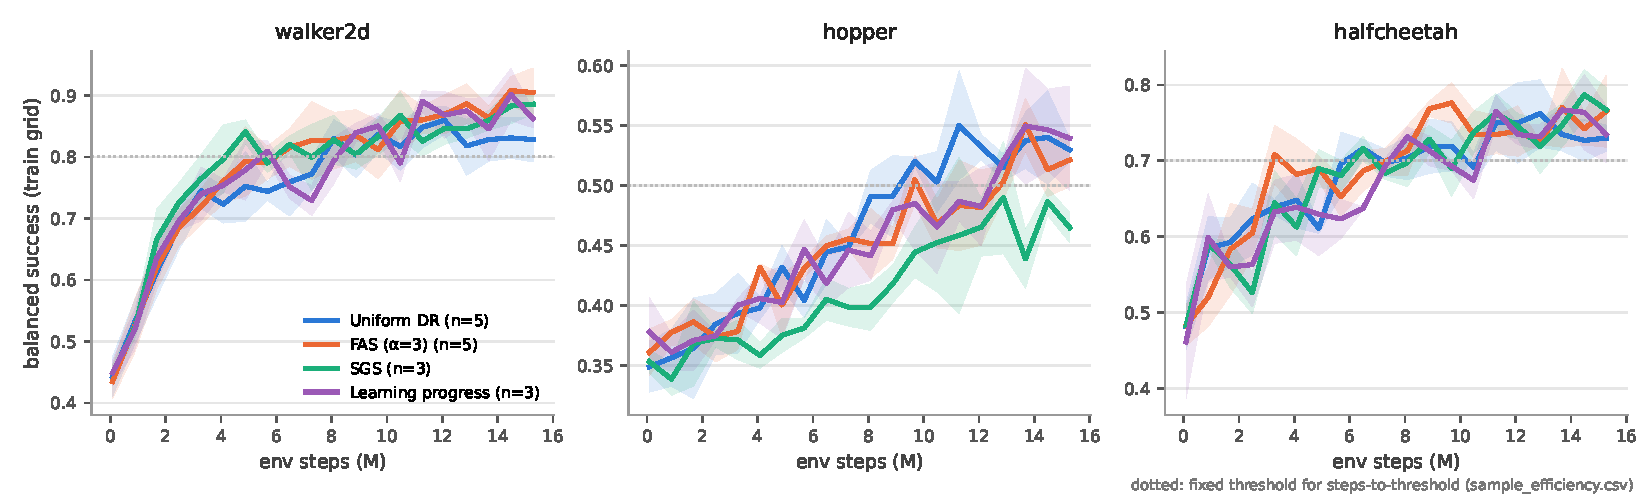
\includegraphics[width=\linewidth]{fig_curves.pdf}
\caption{Balanced success on the training grid during fine-tuning (mean $\pm$ std over seeds). Dotted line: threshold used for steps-to-threshold.}
\label{fig:curves}
\end{figure}

Table~\ref{tab:main} and Fig.~\ref{fig:curves} summarize RQ1.
\textbf{Training under disturbances matters most.} Uniform DR improves on nominal DPPO by 10--14 points on the training grid.
\textbf{\fas{} adds a task-dependent gain.} On walker2d, \fas{} improves train success by 3.9 points ($t=3.8$), OOD success by 4.0 ($t=1.9$), worst-25\% success from 0.498 to 0.576, and AUC from 0.754 to 0.780 ($t=2.8$; median iterations to 0.8 success: 80 vs.\ 100).
On halfcheetah (8 seeds) the gain is smaller: 2.9 points on the training grid ($t=2.0$) and 5.1 on the worst-25\% bins ($t=2.0$), both with bootstrap CIs excluding zero; OOD ($+2.2$) and AUC are within noise. On hopper (6 seeds) \fas{} and uniform DR are within noise ($|t|<1$).
\textbf{\fas{}+LP} is the best method on walker2d: 0.896 train ($t=8.2$), 0.638 worst-25\%, 0.457 OOD, and AUC 0.793 ($t=7.6$); for all four, the 95\% bootstrap CI of the difference to uniform excludes zero.
It is also the best method on halfcheetah: 0.795 train ($t=2.7$), 0.407 worst-25\% ($t=3.2$) and AUC $t=3.8$, all with CIs excluding zero. On hopper it does not help.
Per-bin analysis (as in Fig.~\ref{fig:v3}, right) shows where the gains come from: the bins that uniform DR already solves are nearly identical across methods, and the improvement comes from the frontier bins.

\subsection{RQ2: What governs the exploration--stability trade-off?}
\label{sec:rq2}

\textbf{Sampling strength.} With $\alpha=1$, $\beta=0.5$, \fas{} samples about as evenly as 30 of the 36 bins (effective number of bins $1/\sum_c p(c)^2$) and matches uniform DR (walker2d 0.840).
With $\alpha=3$, $\beta=0.9$ it concentrates on about 12 bins and gains 3.9 points. \fas{} helps only when it actually concentrates.

\textbf{Critic error does not appear to be the bottleneck.} For every bin we roll out the stochastic policy and compare $V(s)$ with the Monte-Carlo return, which is the critic's regression target.\footnote{DPPO treats the time limit as terminal and its critic has no time input, so part of the error ($\approx$0.3 relative) is irreducible; we therefore compare methods, not absolute values.}
\fas{} never increases relative critic error: walker2d 0.319 vs.\ 0.332 for uniform, hopper 0.350 vs.\ 0.360.
The same holds under sparse rewards (below), including on the bins \fas{} keeps failing.
Bins that a method samples more have slightly \emph{lower} error (correlation $-0.1$ to $-0.36$).

\textbf{Reward sparsity amplifies the effect of concentration.} We delay the dense reward: it is accumulated and paid every $K$ steps, which leaves the episode return unchanged (Fig.~\ref{fig:sparse}).
On walker2d, the advantage of \fas{} grows with sparsity: at $K=25$ it is $+5.4$ points ($t=4.5$) on the training grid and $+11.5$ ($t=7.8$) on the worst-25\% bins.
On hopper the sign flips. \fas{} falls behind uniform DR as $K$ grows, by $-2.1$ points at $K=100$ (5 seeds), and its AUC is lower with a 95\% CI that excludes zero ($t=-3.3$).
Since critic error is unchanged, this points to \emph{where} the samples go.

\textbf{Learnability: a prediction fixed before training.} On hopper's main grid, the 300\,N pushes turned out to be far harder than on the other two robots: after fine-tuning, uniform DR is still at about the pretrained success rate on these bins. No method we tried learns them within our budget, yet \fas{} places 46\% of its samples on bins it is currently failing.
This observation motivated a follow-up experiment on a second hopper grid, the \emph{learnable grid}: the same mass and friction values, with pushes of $\{0, 100, 200\}$\,N instead of $\{0, 150, 300\}$\,N.
We chose it by evaluating existing policies (the uniform-DR policy trained on the main grid leaves only 2 of its 36 bins unsolved), and wrote down the prediction that \fas{} beats uniform DR before training on it.
The prediction holds (Fig.~\ref{fig:v3}): over 5 seeds, \fas{} reaches 0.723 vs.\ 0.684 train success ($t=3.5$), 0.358 vs.\ 0.282 on the worst-25\% bins ($t=2.7$), and a higher AUC than uniform DR on every seed ($t=2.6$); all three bootstrap 95\% CIs exclude zero. OOD success is unchanged (0.303 vs.\ 0.307).
All of the gain is on frontier bins (0.49$\to$0.56); solved bins stay at 0.96.
\emph{Answer to RQ2: in our experiments, the trade-off is best explained by whether the conditions \fas{} focuses on are learnable, not by critic stability.} The learnable grid is also easier overall, so this test supports but does not isolate learnability.

\begin{figure}[t]
\centering
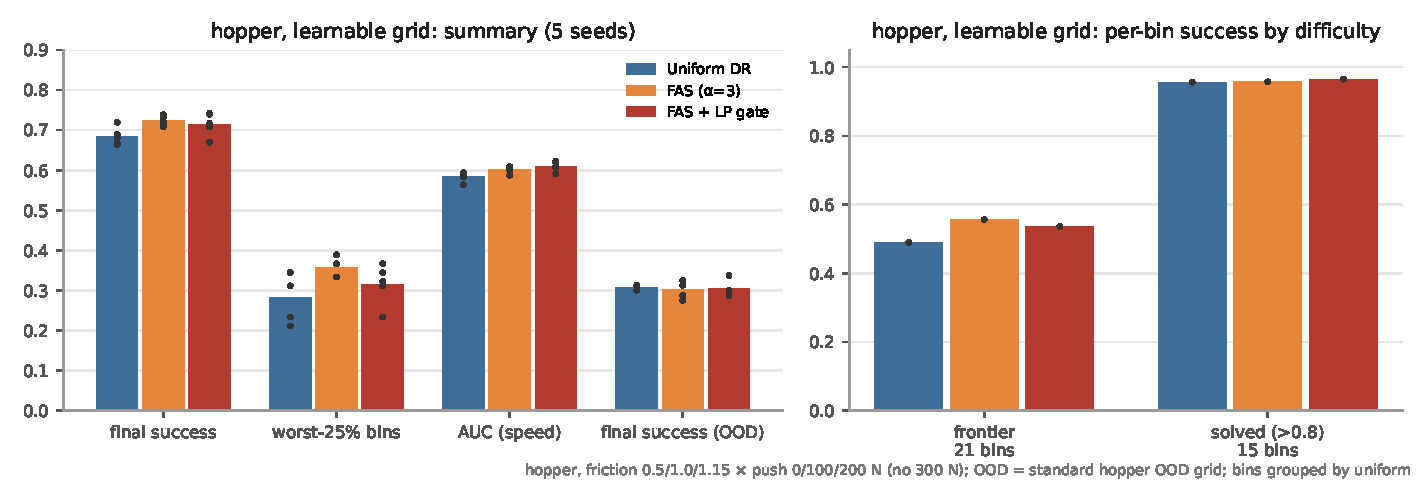
\includegraphics[width=\linewidth]{fig_hopper_v3.pdf}
\caption{Hopper, learnable grid (pushes $\{0, 100, 200\}$\,N; mass and friction as in the main grid). Left: per-seed final success, worst-25\% bins, AUC and OOD success. Right: per-bin success, grouped by the uniform policy's difficulty. 5 seeds.}
\label{fig:v3}
\end{figure}

\begin{figure}[t]
\centering
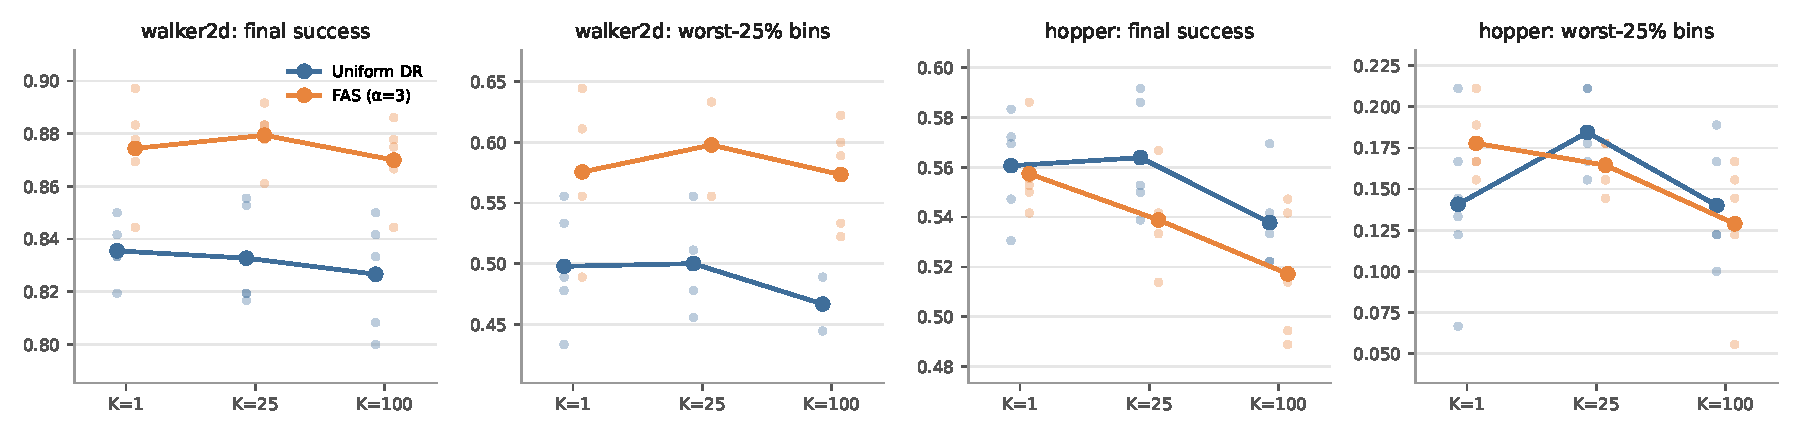
\includegraphics[width=\linewidth]{fig_sparse_compact.pdf}
\caption{Reward sparsity: the dense reward is paid every $K$ environment steps (episode return unchanged). Final success and worst-25\% bins on the training grid; lines show the mean over seeds, faint dots individual seeds. Seeds for $K=1/25/100$: walker2d 5/3/3, hopper 6/3/5.}
\label{fig:sparse}
\end{figure}

\subsection{Comparison with adaptive curricula}
\label{sec:baselines}

SGS matches \fas{} on walker2d and learns fastest there (median 60 iterations to 0.8 success), but it is among the worst methods on hopper (0.496) and no better than uniform DR on halfcheetah. LP lies between uniform DR and \fas{} on walker2d and is within noise of uniform DR elsewhere.
\textbf{PLR is worse than uniform DR} on all three tasks (walker2d 0.790, hopper 0.493, halfcheetah 0.712; $t$ between $-2.9$ and $-3.9$).
PLR samples the \emph{easy} bins: 87\% (walker2d) and 66\% (hopper) of its mass goes to bins that uniform DR already solves, and its sampling probability correlates positively with uniform's per-bin success ($+0.73$/$+0.60$).
A likely reason is that in dense-reward locomotion the positive value loss scales with the return and the episode length, so it tracks how long the policy survives rather than how much it can still learn.
Failure rate is a more direct difficulty signal here, which is consistent with the critic analysis above.

\subsection{RQ3: RL update vs.\ imitating discovered successes}
\label{sec:rq3}

\begin{table}[t]
\centering
\caption{RFT on the successful training episodes of each source run (train / OOD success, mean over source seeds). Source seeds: walker2d 0--2, hopper 3--5, halfcheetah 5--7.}
\label{tab:rft}
\small
\begin{tabular}{llccc}
\toprule
Task & Source of successes & RL policy & RFT & RFT + 60\% D4RL demos \\
\midrule
\multirow{2}{*}{walker2d} & \fas{} run & 0.882 / 0.450 & \textbf{0.820} / \textbf{0.400} & 0.654 / 0.367 \\
& Uniform DR run & 0.831 / 0.400 & 0.752 / 0.383 & 0.635 / 0.350 \\
\midrule
\multirow{2}{*}{hopper} & \fas{} run & 0.550 / 0.296 & 0.468 / \textbf{0.258} & 0.420 / 0.283 \\
& Uniform DR run & 0.568 / 0.283 & \textbf{0.469} / 0.225 & 0.424 / 0.233 \\
\midrule
\multirow{2}{*}{halfcheetah} & \fas{} run & 0.797 / 0.471 & \textbf{0.665} / \textbf{0.383} & 0.620 / 0.312 \\
& Uniform DR run & 0.733 / 0.433 & 0.628 / 0.371 & 0.612 / 0.342 \\
\bottomrule
\end{tabular}
\end{table}

On walker2d, RFT recovers 78--85\% of the RL policy's train-grid gain over the pretrained policy (Table~\ref{tab:rft}); on hopper 43--47\% and on halfcheetah 53--54\%.
\fas{} successes make an equal or better RFT dataset than uniform DR's, presumably because they cover more hard conditions. Successes of the frozen pretrained policy give nothing ($0.454$ vs.\ $0.464$ on walker2d), and mixing in nominal-only demonstrations lowers train success by 2--17 points.
RFT does not fall short because diffusion BC cannot reproduce the RL policy: BC on 100 rollouts per bin of the \emph{final} RL policy, with the same gradient steps, recovers 96--115\% of the gain on all tasks. Most of the gap comes from imitating successes accumulated over training, many from earlier policies: using only the last 50 iterations raises recovery to 71--77\% on hopper and 70--88\% on halfcheetah, but only to 90--94\% on walker2d. Walker2d's early data are not less stale (in action distance to the final policy they are the most stale); rather, walker2d loses the smallest share of its gain to action errors: Gaussian action noise with $\sigma=0.1$ removes 7\% of the RL gain on walker2d, 14\% on hopper (same absolute loss, half the gain) and 48\% on halfcheetah. This separates walker2d from the other two tasks but does not order hopper and halfcheetah, so it is supporting evidence rather than a full account. Keeping only successes with a margin over the success criterion does not help.
\emph{Answer to RQ3: imitation itself is not the bottleneck;} but RFT on accumulated successes is diluted by earlier policies, which costs least on walker2d.

\subsection{LEGO assembly}
\label{sec:lego}
\todo{Teammates: main result table/figure (uniform vs.\ \fas{}), and how it relates to the MuJoCo findings. LEGO has a binary success reward, so \S\ref{sec:rq2} predicts that \fas{} helps if the failing configurations are learnable and hurts if they are not. $\sim$0.5--0.75 page.}

\subsection{Negative results}
\label{sec:negative}
(i) \fas{} gives no gain on hopper's main grid: on its 20 frontier bins, uniform DR, \fas{}, LP and \fas{}+LP all reach about 0.47, and its hardest bins contain a push that no method learns (\S\ref{sec:rq2}).
(ii) A harder walker2d grid (mass up to 1.75, friction down to 0.35, pushes up to 450\,N) does not widen the gap (0.635 vs.\ 0.618, $t=1.8$): when most bins are failing, the failure weights become nearly flat and \fas{} spreads its samples over about 21 bins.
(iii) The LP gate does not detect hopper's unlearnable bins, whose failure rate fluctuates almost as much as that of frontier bins.
(iv) PLR (\S\ref{sec:baselines}).

%===============================================================================
\section{Summary and Future Directions}
\label{sec:conclusion}

Failure-aware sampling is a one-line change to the condition sampler of DPPO. When the conditions a policy fails on are learnable (walker2d, halfcheetah, hopper's learnable grid), it improves robustness and worst-case performance over uniform domain randomization, on walker2d also sample efficiency, and there the improvement grows under sparse reward.
When they are not learnable, it wastes samples, and sparse reward makes this worse.
Critic stability, the risk we worried about most, did not limit \fas{} in our experiments.
The practical lesson is that the condition space must be designed or adapted so that its hard region is reachable.

\textbf{Future directions.}
(1) \emph{Learnability-aware sampling:} the LP gate helps on walker2d but does not detect unlearnable bins; better estimates of learnability, e.g.\ from the success rate of the stochastic policy or from ensemble disagreement, could make \fas{} safe by default.
(2) \emph{Combining \fas{} with ADR:} grow the condition range when the frontier is exhausted and focus within it otherwise.
(3) \emph{Continuous conditions} instead of 36 discrete bins.
(4) \emph{Hybrid RL+RFT:} BC on recent successes recovers most of the RL gain (\S\ref{sec:rq3}), so cheap RFT on the latest \fas{}-collected successes could replace part of the RL updates.
\todo{LEGO-specific future work.}

%===============================================================================
\acknowledgments{\todo{optional}}

{\small\bibliography{references}}

\end{document}
